\documentclass[10pt,onecolumn,letterpaper]{article}

\usepackage{cvpr}
\usepackage{times}
\usepackage{epsfig}
\usepackage{graphicx}
\usepackage{grffile}
\usepackage{amsmath}
\usepackage{amssymb}
\usepackage{amsmath}
\usepackage{amsfonts}
\usepackage{subfigure}
\usepackage{nonfloat}
\usepackage{url}
%\usepackage[colorlinks=true, linkcolor=green, pagebackref]{hyperref}


\usepackage{wrapfig}
\graphicspath{{../report/imgs/}{./imgs/}{./imgs/bigbird/new_turntables/}{./imgs/bigbird/rgb_ims/}} %renders_turn_table_new/}}

\usepackage{xspace}
\renewcommand*{\eg}{e.g.\@\xspace}
\renewcommand*{\ie}{i.e.\@\xspace}
\newcommand*{\ea}{et al.\@\xspace}
\renewcommand*{\vs}{vs.\@\xspace}

\def\cvprPaperID{1437} % *** Enter the CVPR Paper ID here
\def\httilde{\mbox{\tt\raisebox{-.5ex}{\symbol{126}}}}


\title{Structured Prediction of Unobserved Voxels From a Single Depth Image: Supplementary Material}

\begin{document}

\maketitle


%%%%%%%%%%%%%%%%%%%%%%%%%%%%%%%%%%%%%%%%%%%%%%%%%%%%%%%%
\section{Full pipeline of images}


In Figure 1 we show the depth image preprocessing pipeline we use before we make our predictions.
The noisy depth image (b) is smoothed, and missing data is filled (c). 
This makes use of the RGB image in the cross-bilateral filtering, where we use the implementation provided by \cite{silberman-eccv-2012}.
We then use the structured edge detection model from \cite{dollar-iccv-2013} to compute a real-valued edge map (d) for the image, which is finally binarized (e) using the Canny edge hysteresis method \cite{canny-pami-1986}.
\newcommand{\preprocesssubwidth}{0.3\columnwidth}
\begin{figure*}[b]
\begin{tabular}{ccc}
    \centering 
    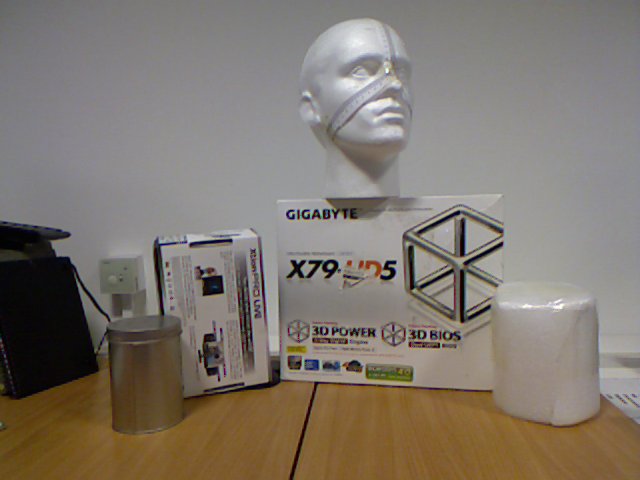
\includegraphics[width=\preprocesssubwidth]{process/preprocess_a} & 
    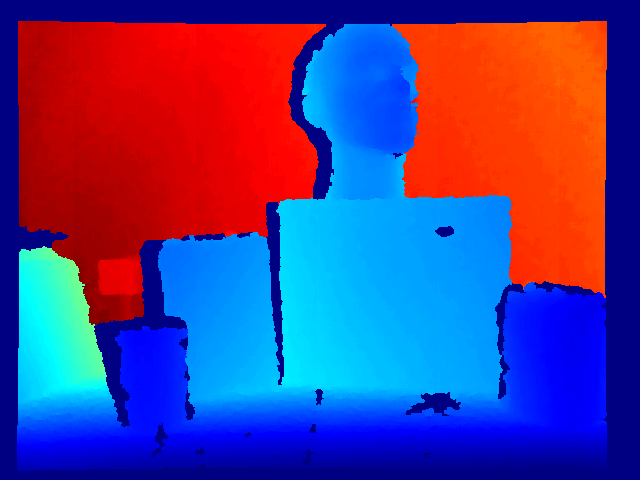
\includegraphics[width=\preprocesssubwidth]{process/preprocess_b} &
    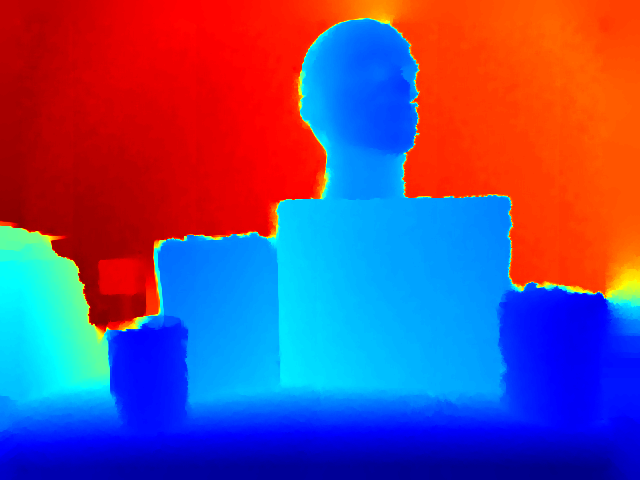
\includegraphics[width=\preprocesssubwidth]{process/preprocess_c} \\ 
    (a) RGB image & (b) Raw depth image & (c) Smoothed depth \\
    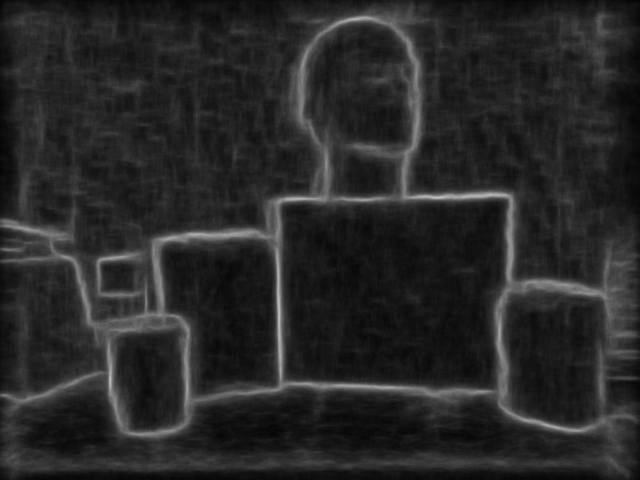
\includegraphics[width=\preprocesssubwidth]{process/preprocess_d} &
    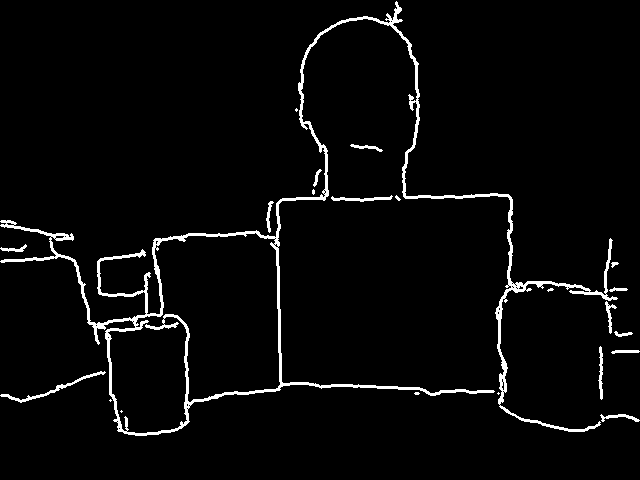
\includegraphics[width=\preprocesssubwidth]{process/preprocess_e} & \\
    (d) Structured edges &
    (e) Binary edge map & \\
\end{tabular}
\vspace{5pt}
\caption{\small Pre-processing pipeline}
\label{fig:preproc}
\end{figure*}


\newpage
%%%%%%%%%%%%%%%%%%%%%%%%%%%%%%%%%%%%%%%%%%%%%%%%%%%%%%%%
\section{`Bigbird' turntable dataset: Additional results}

Figure 2 shows additional results from the Bigbird turntable dataset. 
We note that we are able to gain good reconstructions even where the object suffers from heavy self-occlusions  (e.g. (c) and (d)).
However, where much of the data is missing through the height of the object, we can fail to recover the main bulk (e.g. (f) and (g)).
We note that the baseline algorithms can also perform poorly under such conditions, under- or over- predicting the volume.

\newcommand{\turnheight}{0.12\columnwidth}
\vspace{15pt}


%\begin{figure*}[H]
\begin{tabular}{cccccc}
(a) 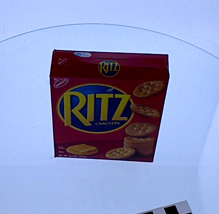
\includegraphics[height=\turnheight, clip=true, trim=20 30 30 5]{ritz_crackers.png} &
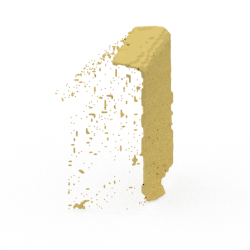
\includegraphics[height=\turnheight, clip=true, trim=60 30 30 5]{ritz_crackers_NP3_0_visible_pixels_view_180.png} &
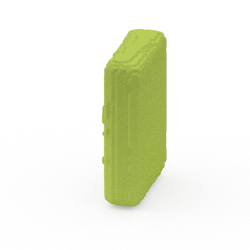
\includegraphics[height=\turnheight, clip=true, trim=60 30 30 5]{ritz_crackers_NP3_0_gt_view_180.png} &
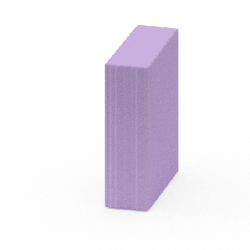
\includegraphics[height=\turnheight, clip=true, trim=60 30 30 5]{ritz_crackers_NP3_0_bb_view_180.png} &
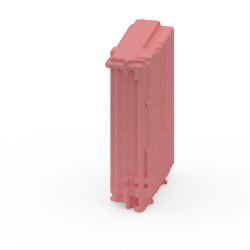
\includegraphics[height=\turnheight, clip=true, trim=60 30 30 5]{ritz_crackers_NP3_0_zheng_view_180.png} &
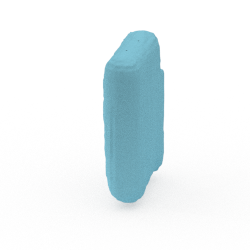
\includegraphics[height=\turnheight, clip=true, trim=60 30 30 5]{ritz_crackers_NP3_0_oma_view_180} \\
(b) 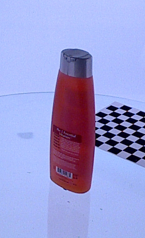
\includegraphics[height=\turnheight, clip=true, trim=20 30 30 5]{vo5_extra_body_volumizing_shampoo.png} &
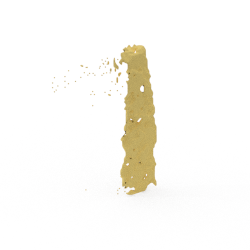
\includegraphics[height=\turnheight, clip=true, trim=60 30 30 5]{vo5_extra_body_volumizing_shampoo_NP2_216_visible_pixels_view_0.png} &
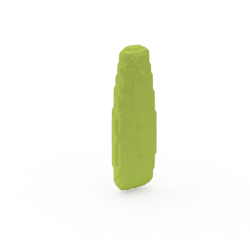
\includegraphics[height=\turnheight, clip=true, trim=60 30 30 5]{vo5_extra_body_volumizing_shampoo_NP2_216_gt_view_0.png} &
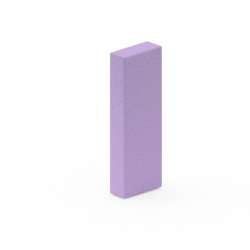
\includegraphics[height=\turnheight, clip=true, trim=60 30 30 5]{vo5_extra_body_volumizing_shampoo_NP2_216_bb_view_0.png} &
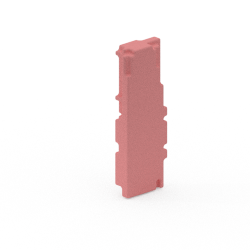
\includegraphics[height=\turnheight, clip=true, trim=60 30 30 5]{vo5_extra_body_volumizing_shampoo_NP2_216_zheng_view_0.png} &
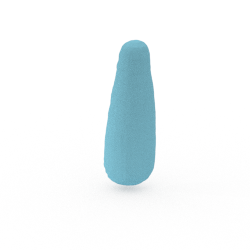
\includegraphics[height=\turnheight, clip=true, trim=60 30 30 5]{vo5_extra_body_volumizing_shampoo_NP2_216_oma_view_0} \\
(c) 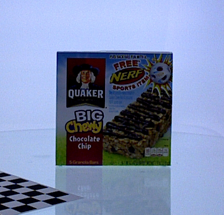
\includegraphics[height=\turnheight, clip=true, trim=20 30 30 5]{quaker_big_chewy_chocolate_chip.png} &
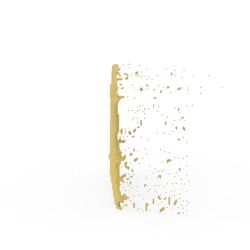
\includegraphics[height=\turnheight, clip=true, trim=60 30 30 5]{quaker_big_chewy_chocolate_chip_NP1_0_visible_pixels_view_0.png} &
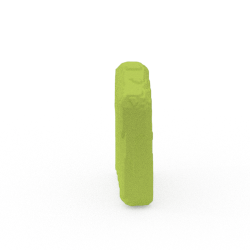
\includegraphics[height=\turnheight, clip=true, trim=60 30 30 5]{quaker_big_chewy_chocolate_chip_NP1_0_gt_view_0.png} &
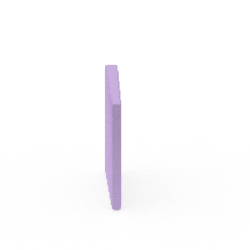
\includegraphics[height=\turnheight, clip=true, trim=60 30 30 5]{quaker_big_chewy_chocolate_chip_NP1_0_bb_view_0.png} &
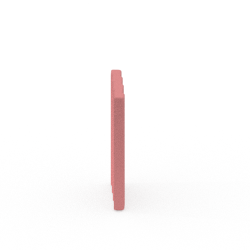
\includegraphics[height=\turnheight, clip=true, trim=60 30 30 5]{quaker_big_chewy_chocolate_chip_NP1_0_zheng_view_0.png} &
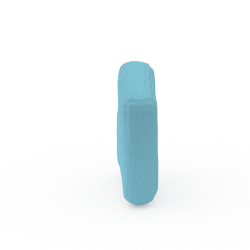
\includegraphics[height=\turnheight, clip=true, trim=60 30 30 5]{quaker_big_chewy_chocolate_chip_NP1_0_oma_view_0} \\
(d) 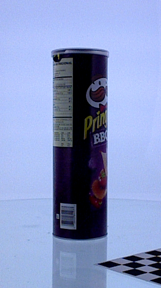
\includegraphics[height=\turnheight, clip=true, trim=20 30 30 5]{pringles_bbq_NP1_312.png} &
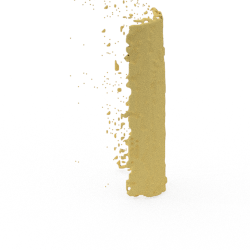
\includegraphics[height=\turnheight, clip=true, trim=60 30 30 5]{pringles_bbq_NP1_312_visible_pixels_view_180.png} &
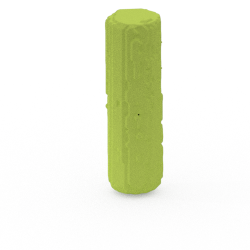
\includegraphics[height=\turnheight, clip=true, trim=60 30 30 5]{pringles_bbq_NP1_312_gt_view_180.png} &
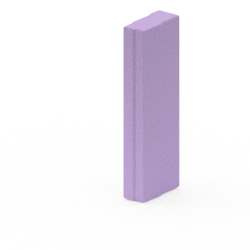
\includegraphics[height=\turnheight, clip=true, trim=60 30 30 5]{pringles_bbq_NP1_312_bb_view_180.png} &
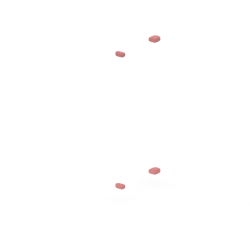
\includegraphics[height=\turnheight, clip=true, trim=60 30 30 5]{pringles_bbq_NP1_312_zheng_view_180.png} &
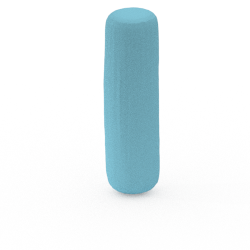
\includegraphics[height=\turnheight, clip=true, trim=60 30 30 5]{pringles_bbq_NP1_312_oma_view_180} \\
% (g) \includegraphics[height=\turnheight, clip=true, trim=20 30 30 5]{pringles_bbq_NP4_0.png} &
% \includegraphics[height=\turnheight, clip=true, trim=60 30 30 5]{pringles_bbq_NP4_0_visible_pixels_view_0.png} &
% \includegraphics[height=\turnheight, clip=true, trim=60 30 30 5]{pringles_bbq_NP4_0_gt_view_0.png} &
% \includegraphics[height=\turnheight, clip=true, trim=60 30 30 5]{pringles_bbq_NP4_0_bb_view_0.png} &
% \includegraphics[height=\turnheight, clip=true, trim=60 30 30 5]{pringles_bbq_NP4_0_zheng_view_0.png} &
% \includegraphics[height=\turnheight, clip=true, trim=60 30 30 5]{pringles_bbq_NP4_0_oma_view_0} \\
(e) 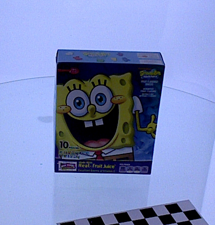
\includegraphics[height=\turnheight, clip=true, trim=20 30 30 5]{spongebob_squarepants_fruit_snaks.png} &
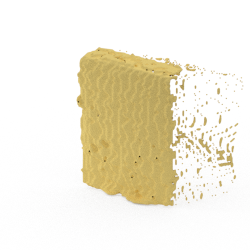
\includegraphics[height=\turnheight, clip=true, trim=60 30 30 5]{spongebob_squarepants_fruit_snaks_NP2_0_visible_pixels_view_90.png} &
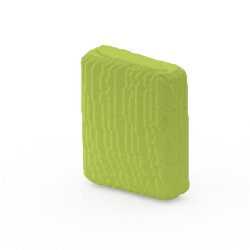
\includegraphics[height=\turnheight, clip=true, trim=60 30 30 5]{spongebob_squarepants_fruit_snaks_NP2_0_gt_view_90.png} &
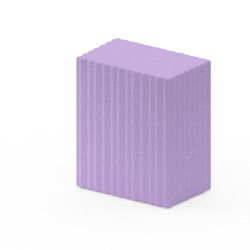
\includegraphics[height=\turnheight, clip=true, trim=60 30 30 5]{spongebob_squarepants_fruit_snaks_NP2_0_bb_view_90.png} &
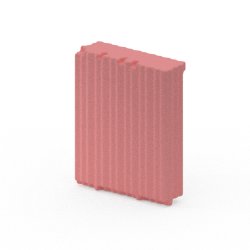
\includegraphics[height=\turnheight, clip=true, trim=60 30 30 5]{spongebob_squarepants_fruit_snaks_NP2_0_zheng_view_90.png} &
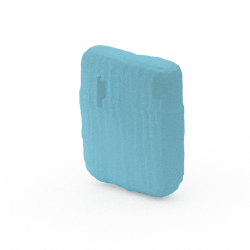
\includegraphics[height=\turnheight, clip=true, trim=60 30 30 5]{spongebob_squarepants_fruit_snaks_NP2_0_oma_view_90} \\
(f) 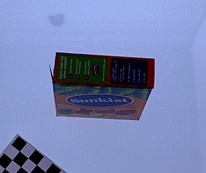
\includegraphics[height=\turnheight, clip=true, trim=20 30 30 5]{sunkist_fruit_snacks_mixed_fruit.png} &
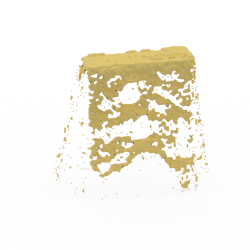
\includegraphics[height=\turnheight, clip=true, trim=60 30 30 5]{sunkist_fruit_snacks_mixed_fruit_NP4_0_visible_pixels_view_90.png} &
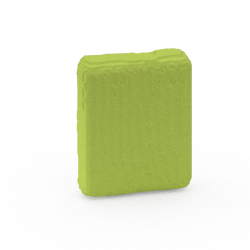
\includegraphics[height=\turnheight, clip=true, trim=60 30 30 5]{sunkist_fruit_snacks_mixed_fruit_NP4_0_gt_view_90.png} &
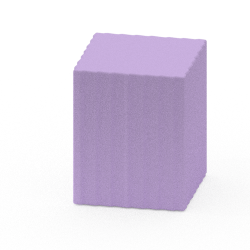
\includegraphics[height=\turnheight, clip=true, trim=60 30 30 5]{sunkist_fruit_snacks_mixed_fruit_NP4_0_bb_view_90.png} &
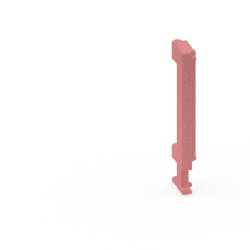
\includegraphics[height=\turnheight, clip=true, trim=60 30 30 5]{sunkist_fruit_snacks_mixed_fruit_NP4_0_zheng_view_90.png} &
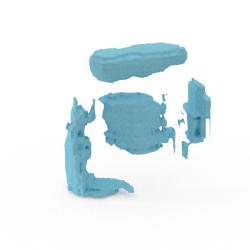
\includegraphics[height=\turnheight, clip=true, trim=60 30 30 5]{sunkist_fruit_snacks_mixed_fruit_NP4_0_oma_view_90} \\
(g) 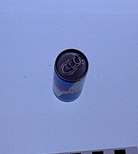
\includegraphics[height=\turnheight, clip=true, trim=20 30 30 5]{red_bull.png} &
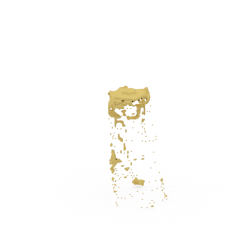
\includegraphics[height=\turnheight, clip=true, trim=60 30 30 5]{red_bull_NP4_0_visible_pixels_view_270.png} &
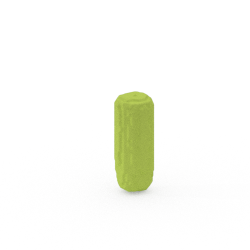
\includegraphics[height=\turnheight, clip=true, trim=60 30 30 5]{red_bull_NP4_0_gt_view_270.png} &
\includegraphics[height=\turnheight, clip=true, trim=60 30 30 5]{red_bull_NP4_0_bb_view_270.png} &
\includegraphics[height=\turnheight, clip=true, trim=60 30 30 5]{red_bull_NP4_0_zheng_view_270.png} &
\includegraphics[height=\turnheight, clip=true, trim=60 30 30 5]{red_bull_NP4_0_oma_view_270} \\
     Input view & Input depth pixels & Ground truth mesh & Bounding box &  Zheng \ea & Our result \\
\end{tabular}
\label{fig:bb}
\vspace{10pt}

%\centering
%{\centering Figure 2. Additional results from the Bigbird dataset}
\centerline{\small Figure 2. Additional results from the Bigbird dataset}

%\raggedright
%\end{figure*}




%    \vspace{5pt}
%     \caption{Results from the Bigbird turntable dataset. 
 %    Each row shows a different object, while each column shows the result of a different algorithm.
 %     The first column shows the RGB image of the input view, while the second column shows the reprojected input depth pixels from a side view.
 %    The following columns, all shown from the same viewpoint as the input depth pixels view, demonstrate the different baselines and algorithm variants. 
 %     More views and objects can be seen in the supplementary material.
 %%    \label{fig:turntable_qual}
   %  }


\newpage

\section{Slices through the TSDF}

For most of our images, we have displayed the zero level-set from the truncated signed distance function (TSDF).
However, the underlying TSDF could be useful for some application.
It additionally provides some introspection to reveal the inner workings of the algorithm.
We also note that using marching cubes to find the level set is a fairly naive version of regularization.

The images in Figures 3 and 4 show slices through the TSDF volume at different heights in a prediction.
These test scenes fall well outside the scope of our training data, which was much smaller objects on a turntable.
However, these images show the ability of our algorithm to degrade gracefully in the presence of novel types of data.
It can be seen that some regions are predicted to be occupied (red regions) while actually landing in a region known to be empty, given the camera image. Sometimes this occurs where predictions are made from points above or below the slice being viewed.
We have not in these images made any attempt to remove these regions.

\newcommand{\imheight}{0.17\columnwidth}

\centering
\vspace{10pt}
\begin{tabular}{cc}
\centering
\includegraphics[height=\imheight]{real/head/rgb_00050.png} &
\includegraphics[height=\imheight]{real/head/slice_00050.png} \\
\includegraphics[height=\imheight]{real/head/rgb_00080.png} &
\includegraphics[height=\imheight]{real/head/slice_00080.png} \\
\includegraphics[height=\imheight]{real/head/rgb_00110.png} &
\includegraphics[height=\imheight]{real/head/slice_00110.png} \\
\includegraphics[height=\imheight]{real/head/rgb_00150.png} &
\includegraphics[height=\imheight]{real/head/slice_00150.png} \\
\includegraphics[height=\imheight]{real/head/rgb_00170.png} &
\includegraphics[height=\imheight]{real/head/slice_00170.png} 
\end{tabular}
\vspace{10pt}

{\centering \small Figure 3. Slices through a TSDF prediction. The black line on the raw image on the left of each image pair indicates the height of the slice, while the image on the right shows the values of the TSDF.
The TSDF values range from -3cm (red) to +3cm (blue).
The zero level-set falls in the middle of the white region.
The green dots show the position of the raw Kinect input in the indicated region.
}
\vspace{10pt}


\begin{tabular}{cc}
\centering
\includegraphics[height=\imheight]{real/statue/rgb_00050.png} &
\includegraphics[height=\imheight]{real/statue/slice_00050.png} \\
\includegraphics[height=\imheight]{real/statue/rgb_00080.png} &
\includegraphics[height=\imheight]{real/statue/slice_00080.png} \\
\includegraphics[height=\imheight]{real/statue/rgb_00110.png} &
\includegraphics[height=\imheight]{real/statue/slice_00110.png} \\
\includegraphics[height=\imheight]{real/statue/rgb_00150.png} &
\includegraphics[height=\imheight]{real/statue/slice_00150.png} \\
\includegraphics[height=\imheight]{real/statue/rgb_00200.png} &
\includegraphics[height=\imheight]{real/statue/slice_00200.png}
\end{tabular}
\vspace{10pt}

{\centering \small Figure 4. Slices through a TSDF prediction. Colors and images are as described in the caption of Figure 3.}


{\small
\bibliographystyle{ieee}
\bibliography{../report/bibtex/strings.bib,../report/bibtex/main.bib,../report/bibtex/crossrefs.bib}
}



\end{document}